%!TEX TS-program = xelatex
\documentclass[12pt]{article}
\usepackage[noblocks]{authblk}
\usepackage{amsmath, amssymb}
\usepackage{booktabs}
\usepackage{longtable}
\usepackage{array}
\usepackage{pifont}

\usepackage{lineno}
\renewcommand{\linenumberfont}{\normalfont\bfseries\small}
%\linenumbers
\usepackage{fontspec}
\PassOptionsToPackage{hyphens}{url}\usepackage{hyperref}

\setmainfont{Georgia}
\usepackage[utf8]{inputenc}
\usepackage[letterpaper, margin=2cm]{geometry}
\usepackage{soul}
\renewcommand{\baselinestretch}{2}

\usepackage{fixltx2e}
\usepackage{gensymb}
\usepackage[export]{adjustbox}

\date{}

\usepackage{fancyhdr}
\usepackage[shortlabels]{enumitem}

% Only number sections (S1, S2, S3) and subsections (S1.1, S2.1, etc.).
% Subsubsections will NOT be numbered (no S3.1.7).
\setcounter{secnumdepth}{2}

\usepackage[compact]{titlesec}
\titlespacing{\section}{0pt}{-1.0ex}{-1.0ex}
\titlespacing{\subsection}{0pt}{1ex}{0ex}
\titlespacing{\subsubsection}{0pt}{1.2ex}{0.2ex}

\titleformat{\section}{\normalfont\large\bfseries}{\thesection}{1em}{}
\titleformat{\subsection}{\normalfont\normalsize\bfseries}{\thesubsection}{1em}{}
\titleformat{\subsubsection}{\normalfont\normalsize\bfseries}{}{0pt}{}

\usepackage{natbib}
\bibliographystyle{ecology}
\usepackage{wrapfig}
\usepackage{graphicx}
\usepackage{caption}
\usepackage{subcaption}
\usepackage[font=small,labelfont=bf]{caption}
\graphicspath{ {../figures/original_v1_figures/} {../figures/new_physical_model_figures/} {../figures/new_dnn_and_ablation_figures/} }

\makeatletter
\renewcommand \thesection{S\@arabic\c@section}
\renewcommand\thetable{S\@arabic\c@table}
\renewcommand \thefigure{S\@arabic\c@figure}
\renewcommand\theequation{S\@arabic\c@equation}
\makeatother

\setlength{\parskip}{0.5em}
\emergencystretch=2.5em
\tolerance=2000

\begin{document}

\title{Supplementary materials\newline Spatially Aware Deep Learning for Microclimate Prediction from High-Resolution Geospatial Imagery}

\author[1]{\normalsize Idan Sulami}
\author[1]{\normalsize Alon Itzkovitch}
\author[2]{\normalsize Michael R. Kearney}
\author[3]{\normalsize Moni Shahar}
\author[1,*]{\normalsize Ofir Levy}

\affil[1]{\normalsize Tel Aviv University, Faculty of Life Sciences, School of Zoology, Tel Aviv, Israel}
\affil[2]{\normalsize School of BioSciences, The University of Melbourne, Melbourne, Victoria, Australia}
\affil[3]{\normalsize Tel Aviv University, Center for Artificial Intelligence \& Data Science, Tel Aviv, Israel}

\maketitle

\newpage
%TC:ignore
\section{Maps Development for Microclimate Modelling}

\subsection{Solar Radiation}
\noindent
Solar radiation was estimated as the total incoming shortwave radiation (direct and diffuse) reaching each pixel, accounting for local surface orientation. This layer was derived from the Digital Surface Model (DSM) by first calculating pixel-level slope and aspect using the GRASS GIS module \textit{r.slope.aspect}. These terrain parameters were then used as inputs to the \textit{r.sun} module to compute spatially explicit solar radiation values.

The \textit{r.sun} calculations require information on solar geometry, including the day of year and solar time, which were obtained using the \textit{getSunlightTimes} function from the \textit{suncalc} R package \citep{Thieurmel_2022}. Because \textit{r.sun} estimates solar radiation under clear-sky conditions, modeled values were adjusted to account for cloud cover. This correction was applied by scaling the radiation map:
\begin{equation}
S_{\text{corrected}}(x, y) = S_{\text{clear-sky}}(x, y) \cdot C_{\text{cloud}}
\end{equation}
where the cloud correction scaling factor $C_{\text{cloud}}$ is derived as:
\begin{equation}
C_{\text{cloud}} = \frac{S_{\text{measured}}}{\max_{\{x, y \mid \text{slope}(x, y) < 0.1^{\circ}\}} S_{\text{clear-sky}}(x, y)}
\end{equation}
where $S_{\text{measured}}$ is the solar radiation measured at the weather station, and the denominator represents the maximum modeled clear-sky solar radiation over near-horizontal surfaces (slope $< 0.1^{\circ}$) within the mapping area.

\subsection{Shade}
\noindent
Shade was represented as a binary spatial layer, with pixels classified as either shaded (1) or unshaded (0). This layer was derived using the \textit{r.sun} module in GRASS GIS by computing a solar incidence map, which describes the angle at which direct solar radiation reaches each pixel. Pixels assigned NULL values in the incidence output correspond to locations receiving no direct sunlight at the time of image acquisition and were therefore classified as shaded.

Shaded pixels in this analysis represent bare ground surfaces that were temporarily shaded by nearby landscape elements, such as rocks, shrubs, or local topographic relief, as determined by solar position during the survey. Areas beneath dense vegetation canopy were excluded from the dataset.

\subsection{Skyview}
\noindent
Skyview was quantified as the skyview factor, defined as the proportion of visible sky at each pixel constrained by surrounding terrain and surface features such as rocks, shrubs, and trees. This layer was calculated using the \textit{r.skyview} module in GRASS GIS. In microclimate modeling, the skyview factor influences the balance of longwave radiation received at the surface, with lower values indicating greater obstruction by surrounding features and higher values corresponding to more open conditions. Skyview values range from 0 to 1, where values close to 0 indicate surfaces that are largely enclosed by surrounding features and values close to 1 indicate fully exposed locations with an unobstructed view of the sky.

\subsection{Vegetation Cover}
\noindent
Vegetation cover was quantified from the RGB orthophotos using the Triangular Greenness Index (TGI), calculated for each pixel as a proxy for chlorophyll content \citep{hunt_2013}:
\begin{equation}
\text{TGI} = -0.5 \cdot \left[ (\lambda_{\text{Red}} - \lambda_{\text{Blue}})(R_{\text{Red}} - R_{\text{Green}}) - (\lambda_{\text{Red}} - \lambda_{\text{Green}})(R_{\text{Red}} - R_{\text{Blue}}) \right]
\end{equation}
Given the sensor band centers ($\lambda_{\text{Red}} = 670\text{ nm}$, $\lambda_{\text{Green}} = 550\text{ nm}$, $\lambda_{\text{Blue}} = 480\text{ nm}$), this equation simplifies to:
\begin{equation}
\text{TGI} = R_{\text{Green}} - 0.39 \cdot R_{\text{Red}} - 0.61 \cdot R_{\text{Blue}}
\end{equation}
where $R_{\text{Red}}$, $R_{\text{Green}}$, and $R_{\text{Blue}}$ represent the digital numbers (reflectances) of the red, green, and blue bands, respectively.

\subsection{Height}
\noindent
Height was quantified as the local elevation of surface features relative to the surrounding ground at each pixel. This layer was derived by calculating the difference between the Digital Surface Model (DSM), which captures the elevation of surface features such as rocks, terraces, and low vegetation, and the Digital Terrain Model (DTM), which represents the underlying ground surface. The resulting difference provides an estimate of object height and microtopographic variation across the landscape \citep[following][]{duffy_2021}. Values approach zero in open areas and increase where surface features protrude above the ground.


\section{Deep Learning Model Architecture and Data Preprocessing}

\noindent The model is a neural network \citep{lecun_2015}: a chain of simple arithmetic operations whose internal numbers (``parameters'') are tuned automatically during training so that its output matches the drone-measured ground temperatures. Each component of the model is first described in words and then defined by its equations.

\subsection{Data Normalization and Centering}

\noindent The inputs differ by orders of magnitude (for example, solar radiation exceeds $800~\text{W m}^{-2}$, whereas the vegetation greenness index is of order $10^{-2}$), which would allow large-valued inputs to dominate training. We therefore standardised every input, namely the five spatial layers and the eight weather variables, using the $z$-score transformation
\begin{equation} \label{eq:zscore}
Z_k = \frac{X_k - \mu_k}{\sigma_k},
\end{equation}
where $\mu_k$ and $\sigma_k$ are the mean and standard deviation of feature $k$ in the training set.

The temperatures the model learns to predict are expressed relative to a local reference. Each thermal map is divided into sub-maps, and within each sub-map we compute the mean temperature of flat, exposed bare sand (pixels that are not shaded and have no object taller than 20~cm). This open-sand reference is subtracted from every pixel, so the model learns to predict ``how much warmer or cooler than the nearby open sand'' rather than the absolute temperature of the day. This removes the overall level of each flight (a cool morning versus a hot afternoon) and lets the model concentrate on the pattern of warm and cool spots: the contrast between sunlit and shaded ground. The reference is added back after prediction to recover the physical temperature.

For each sub-map $s$, the open-sand reference is $T_{\text{ref}}(s) = \overline{T_g}\,\big|\,\text{SHD}=0,\ H<0.20~\text{m}$ (falling back to all unshaded pixels, then to all valid pixels, if fewer than 50 or 10 pixels qualify). Targets are anchored to it and the reference is restored after prediction:
\begin{equation}
\tilde{T}_g^{\text{target}}(s) = T_g^{\text{target}}(s) - T_{\text{ref}}(s), \qquad
T_g^{\text{pred}}(s) = \tilde{T}_g^{\text{pred}}(s) + T_{\text{ref}}(s).
\end{equation}

\subsection{Network Architecture (\texttt{FullResDilatedCNN})}

\noindent The architecture was designed to answer one question: how far away do rocks, shrubs and relief still influence the ground temperature at a given spot? To answer it, we trained the same model on map tiles of increasing size around the target pixel, from a single pixel up to a square $12.2$~m across. Each tile is a square centred on the target pixel, and the pixel size is 15~cm; the nine tile sizes are listed below.

\begin{center}
\begin{tabular}{lcc}
\hline
Tile (pixels) & Side length (m) & Role \\
\hline
$1\times1$ & 0.15 & Point baseline (no neighbourhood) \\
$5\times5$ & 0.75 & \\
$9\times9$ & 1.35 & \\
$15\times15$ & 2.25 & \\
$21\times21$ & 3.15 & \\
$31\times31$ & 4.65 & \\
$47\times47$ & 7.05 & \\
$63\times63$ & 9.45 & \\
$81\times81$ & 12.15 & Largest neighbourhood \\
\hline
\end{tabular}
\end{center}

A valid comparison across tile sizes requires that model capacity remains constant. In many image networks, covering a larger area requires additional layers or a larger dense layer after the feature maps are flattened, as in VGG \citep{simonyan_2015}, so the number of adjustable parameters grows with input size. If such a model performed better on larger tiles, it would be impossible to determine whether the wider landscape carried useful information or whether the larger model simply had more capacity to memorise the training data. We therefore designed the network to have the same number of parameters (55,729) at every tile size, so that any change in accuracy with tile size can be attributed to the landscape itself.

The network (\texttt{FullResDilatedCNN}) is a convolutional neural network that predicts the ground temperature of a single target pixel. Its inputs are a square tile of five map layers centred on the target pixel (object height, shade, solar radiation, skyview factor and vegetation greenness, TGI) and eight weather-station readings for the time of the flight (wind speed, wind direction, air temperature, relative humidity, dew point, air pressure, solar radiation and the ground temperature at the station; Table~1 in the main text). The five map layers are identical to those used by the physical model (Section S3), whereas the weather inputs overlap only partly: the physical model additionally requires albedo and soil temperature and moisture, which the network does not use. The network first converts the map tile into a summary of the terrain around every pixel of the tile. It then adjusts this summary according to the weather, extracts the summary at the target pixel together with tile-wide averages and maxima, and combines these into a single predicted temperature difference from the local open-sand reference. The following subsections describe each of these operations, which are illustrated in Fig.~3 of the main text.



\subsubsection{Building the Terrain Summary (Six Filtering Layers)}
\noindent Six convolutional layers, applied one after another, convert the five-layer tile into a summary of the surrounding terrain. A convolutional layer slides a small window of learned weights (a filter) across its input maps and, at every pixel, combines the values within the window, across all input maps, into one new number. A filter applied at every pixel yields one new map, and each of our layers applies 32 different filters, so it outputs 32 maps, called channels. The first layer takes the five map layers as input, and each later layer takes the 32 maps produced by the layer before it. The number 32 is therefore the width of each layer, not the number of layers, and only the 32 maps of the sixth layer are passed on as the terrain summary. We used 32 filters per layer to keep the network small enough that it cannot simply memorise the training tiles, because the number of parameters grows with the square of the number of filters; other numbers of filters were not tested. Stacking layers allows the network to recognise progressively larger patterns, such as a shadow edge adjacent to a boulder. Two design choices distinguish this network from image-classification networks such as VGG \citep{simonyan_2015} and ResNet \citep{he_2016}.

First, the map is never reduced in size. Classification networks progressively coarsen their feature maps through pooling or strided convolution (ResNet-18, for example, reduces the map by a factor of 4 in its first layers and by a factor of 32 overall). This builds tolerance to the exact position of an object, which benefits classification but would be detrimental here, because coarsening blurs the sharp edge of a small shadow and erases a narrow rock. Every layer of our network therefore retains the original 15~cm pixel grid.

Second, to extend the area considered around each pixel without reducing the map, the layers use dilated convolutions \citep{yu_2016}. A standard $3\times3$ filter combines a pixel with its eight immediate neighbours. A filter with dilation rate 2 samples the same nine positions at every second pixel, and one with dilation rate 16 samples positions 16 pixels apart. Widening the gaps enlarges the area covered by a layer without adding parameters. With dilation rates of 1, 1, 2, 4, 8 and 16, the field of view of the final layer (its receptive field) is $1 + 2(1+1+2+4+8+16) = 65$ pixels, or about 10~m, across. We chose six layers so that this field of view approximates the scale of the largest tiles: it nearly spans the $63\times63$ tile (9.5~m) but only about 80\% of the width of the $81\times81$ tile (12.2~m). In the $81\times81$ tile, the features of the centre pixel therefore do not encompass a ring about 8 pixels (1.2~m) wide at the tile edge, which reaches the prediction only through the tile-wide average and maximum. Other numbers of layers were not tested.

The information available to these layers is limited by the size of the tile. Positions that fall outside the tile are filled with zeros, which after standardisation corresponds to the average of the training data, so a tile can never supply more information than it contains, even though the layers have a 65-pixel field of view. In a $5\times5$ tile, whose pixels are at most 4 pixels apart, the layers with dilation rates 8 and 16 sample only the pixel itself and act as per-pixel combinations of the 32 maps, and the layer with dilation rate 4 samples only the opposite edge of the tile. Tiles are not padded to a common size: each tile size is a separately trained model that receives tiles of exactly that size.

\noindent Formally, the six layers each have 32 channels, $3\times3$ kernels and dilation rates $d \in \{1, 1, 2, 4, 8, 16\}$. With input tile $X \in \mathbb{R}^{5 \times H \times W}$,
\begin{align}
F_1 &= \text{ReLU}\left(\text{GroupNorm}\left(\text{Conv}_1(X, d_1=1)\right)\right), \\
F_l &= \text{ReLU}\left(\text{GroupNorm}\left(\text{Conv}_l(F_{l-1}, d_l)\right)\right), \quad l = 2,\dots,6,
\end{align}
with every $F_l \in \mathbb{R}^{32 \times H \times W}$. Group Normalization \citep{wu_2018} standardises the activations within groups of channels (here 8 groups of 4), independently of batch size, and the rectified linear unit (ReLU; \citealt{nair_2010}) sets negative values to zero, which allows the layers to represent nonlinear relationships. Neither operation extends the spatial reach. The output $F_6$ is the terrain summary used in the next subsection.

\subsubsection{Adjusting the Terrain Summary for the Weather}
\noindent The weather readings modulate the terrain summary rather than being appended to it, because the same shadow cools the ground by different amounts under different conditions. If the weather were added only at the final stage, the model could use it merely as an identifier of the type of day. Instead, we used feature-wise linear modulation (FiLM; \citealt{perez_2018}), a conditioning mechanism originally developed for visual question answering, in which a question modulates the features extracted from an image. Here, a small auxiliary network reads the eight weather values and outputs, for each of the 32 summary channels, a multiplicative scaling factor and an additive shift. This network has one hidden layer with a hyperbolic tangent (tanh) activation, a smooth, bounded nonlinearity that allows the effect of the weather on the terrain to be nonlinear. We used 16 hidden units to keep this pathway small (about 2\% of all parameters); other activation functions and numbers of hidden units were not tested. Hot, still, sunny conditions can thus amplify the channels that encode shading, whereas cool, windy or humid conditions attenuate them. At the start of training the adjustment is neutral, and the model learns from the data how strongly the weather should matter.

\noindent Formally, a two-layer network with 16 hidden tanh units (1,232 parameters; output weights initialised to zero so that $\gamma = \beta = 0$ at the start of training) maps the weather vector $M \in \mathbb{R}^8$ to a scale $\gamma \in \mathbb{R}^{32}$ and shift $\beta \in \mathbb{R}^{32}$:
\begin{equation}
[\gamma, \beta] = W_{\text{met},2} \tanh\left(W_{\text{met},1} M + b_{\text{met},1}\right) + b_{\text{met},2},
\end{equation}
which are applied to every pixel $(i,j)$ of every channel $c$ of the terrain summary, so that the scaling factor $1+\tanh(\gamma_c)$ lies between 0 and 2:
\begin{equation}
F_{\text{modulated}}(c, i, j) = F_6(c, i, j) \cdot \left(1 + \tanh(\gamma_c)\right) + \beta_c.
\end{equation}

\subsubsection{Reading the Centre Pixel and Its Surroundings}
\noindent The weather-adjusted terrain summary is a map with 32 values at every pixel of the tile, whereas the final prediction layers need a list of numbers whose length is the same for every tile size. This fixed length is what keeps the number of parameters constant. We therefore reduce the map to 101 numbers that describe the target pixel and its setting. Each of the 32 values at a pixel is a learned descriptor of the terrain within about 10~m of that pixel, and its meaning is determined during training.

Three groups of numbers are taken from this map. The first group is the 32 values at the centre pixel, which describe the terrain around the target pixel itself. The second and third groups are the mean and the maximum of each of the 32 values over all pixels of the tile (global average and global maximum pooling; \citealt{lin_2014}), giving 32 numbers each. They describe the broader setting of the target pixel, for example whether the tile is a uniform sand plain or a rugged boulder field, and how strongly the most extreme location in the tile expresses each descriptor.

The fourth group, of five numbers, does not pass through the filtering layers. It is the original value of each of the five map layers (height, shade, solar radiation, skyview factor and TGI) at the centre pixel, copied directly from the input. Each filtering layer combines a pixel with its neighbours, so the exact condition of the target pixel, such as whether it is shaded at that moment, could otherwise be blurred. The direct copy ensures that the network always has this information unaltered. In total, the four groups contain $32 + 32 + 32 + 5 = 101$ numbers. For the $1\times1$ tile, the centre values, the mean and the maximum are identical.

\noindent Formally, with $c_H = \lfloor H/2 \rfloor$ and $c_W = \lfloor W/2 \rfloor$ the indices of the centre pixel,
\begin{align}
F_{\text{center}} &= F_{\text{modulated}}[:, c_H, c_W] \in \mathbb{R}^{32}, &
X_{\text{center}} &= X[:, c_H, c_W] \in \mathbb{R}^{5}, \\
F_{\text{mean}} &= \frac{1}{HW} \sum_{i,j} F_{\text{modulated}}[:, i, j] \in \mathbb{R}^{32}, &
F_{\text{max}} &= \max_{i,j} F_{\text{modulated}}[:, i, j] \in \mathbb{R}^{32}.
\end{align}

\subsubsection{The Final Temperature Calculation}
\noindent The four groups of numbers described above are concatenated into a list of 101 numbers and passed through a fully connected network with one hidden layer of 64 units and ReLU activation, followed by a single output unit: the predicted temperature difference from the local open-sand reference. Adding the reference back gives the ground temperature at the centre pixel.

For the single-pixel baseline, the tile contains only the target pixel, and the model and its parameter count are unchanged. This baseline tells us how well temperature can be predicted from on-site information alone, which serves as the reference against which the benefit of each larger neighbourhood is measured.

\noindent Formally,
\begin{equation}
V_{\text{combined}} = \left[ F_{\text{center}} ; F_{\text{mean}} ; F_{\text{max}} ; X_{\text{center}} \right] \in \mathbb{R}^{101}, \qquad
\tilde{T}_g^{\text{pred}} = W_2 \max\left(0, W_1 V_{\text{combined}} + b_1\right) + b_2,
\end{equation}
with $W_1 \in \mathbb{R}^{64 \times 101}$, $b_1 \in \mathbb{R}^{64}$, $W_2 \in \mathbb{R}^{1 \times 64}$ and $b_2 \in \mathbb{R}$. The matrices $W_1$ and $W_2$ are the weights, and the vector $b_1$ and the number $b_2$ are the offsets (biases), of the hidden and output layers, respectively. Like all other weights and offsets of the network, including the filters of the convolutional layers and the matrices $W_{\text{met},1}$ and $W_{\text{met},2}$ of the weather network, they are not set by hand. They are initialised with small random values and adjusted during training to minimise the difference between predicted and measured temperatures. They are needed because the way in which terrain, weather and ground temperature combine is not known in advance, and learning these values from the data allows the network to find the combinations that best predict temperature. Because no layer's size depends on $H$ or $W$, the parameter count is 55,729 for every tile size from $1\times1$ to $81\times81$.


\subsection{Anchored Evaluation and Scene-Level Offsets on Held-Out Flights}

\noindent The target of the network is the temperature difference from the open-ground mean of the same submap (Section S2.1), so the true scene-level anomaly of open ground is zero by construction. A trained network can nonetheless shift all predictions of a scene by a constant, because the eight weather readings are identical for every tile of a flight and the mapping from this vector to a baseline temperature is learned from only 23 flights. On held-out flights whose weather vector lies outside the training distribution this mapping extrapolates, and each tile-size model (and each random seed) extrapolates differently. In our test set, the five flights with the largest offsets (23.9.19 at 06:10, 07:00 and 16:10; 31.05.21 at 17:12 and 18:05) were the five flights with northerly winds (252--354$^\circ$), whereas all 23 training flights had wind directions between 10$^\circ$ and 199$^\circ$ (Table~\ref{table:flights}); wind direction enters the network as a linearly standardised angle, so a wind from 354$^\circ$ is 5.6 standard deviations from the training mean although it is meteorologically the same as a wind from 6$^\circ$. Replacing only the wind-direction input of these flights by a value inside the training range removed most of the offset without retraining, and on the validation blocks of the training flights, including the dawn and dusk flights, the offset was below 0.5$^\circ$C at every tile size. The offsets were therefore a property of the weather pathway of the network on unseen weather, not of the spatial information in the tiles, and were unrelated to time of day except through the coincidence of wind direction with daypart in our test flights.

Because such an offset is added, squared, to every pixel of a submap, the unanchored MSE of the morning and evening flights was dominated by it (squared offset of 6--9 $^\circ$C$^2$ in the morning and 3--14 $^\circ$C$^2$ in the evening, against a within-scene error of about 1 $^\circ$C$^2$), and its dependence on tile size (largest for tiles of 9--31 pixels, whose networks were the most sensitive to the weather vector) produced an apparent increase of error with tile size at these times. To isolate the within-scene component that spatial context can inform, all errors in the main text are computed after subtracting, from the predictions of each submap, the mean prediction over its unshaded, low open-ground test pixels, i.e. the same operation that defines the target. This uses no observed temperatures and corresponds to reporting predicted temperatures relative to the open sand of the same scene, which is how the target is defined. The scene-level offset is reported separately as the submap bias. Across dayparts and microhabitats, the anchored errors are flat in tile size in the morning and evening and decrease with tile size at midday, and are close to the spatial variance of the observed anomalies in the morning and evening (0.7--1.0 $^\circ$C$^2$), when the ground surface is nearly isothermal relative to the open-sand reference. The evaluation code (\texttt{evaluate\_on\_test\_blocks.py}) writes both the unanchored and the anchored errors and the submap bias, and the diagnostic scripts are in \texttt{final\_model/diagnostics\_dawn\_dusk/} of the repository.

\begin{figure}[!ht]
\centering
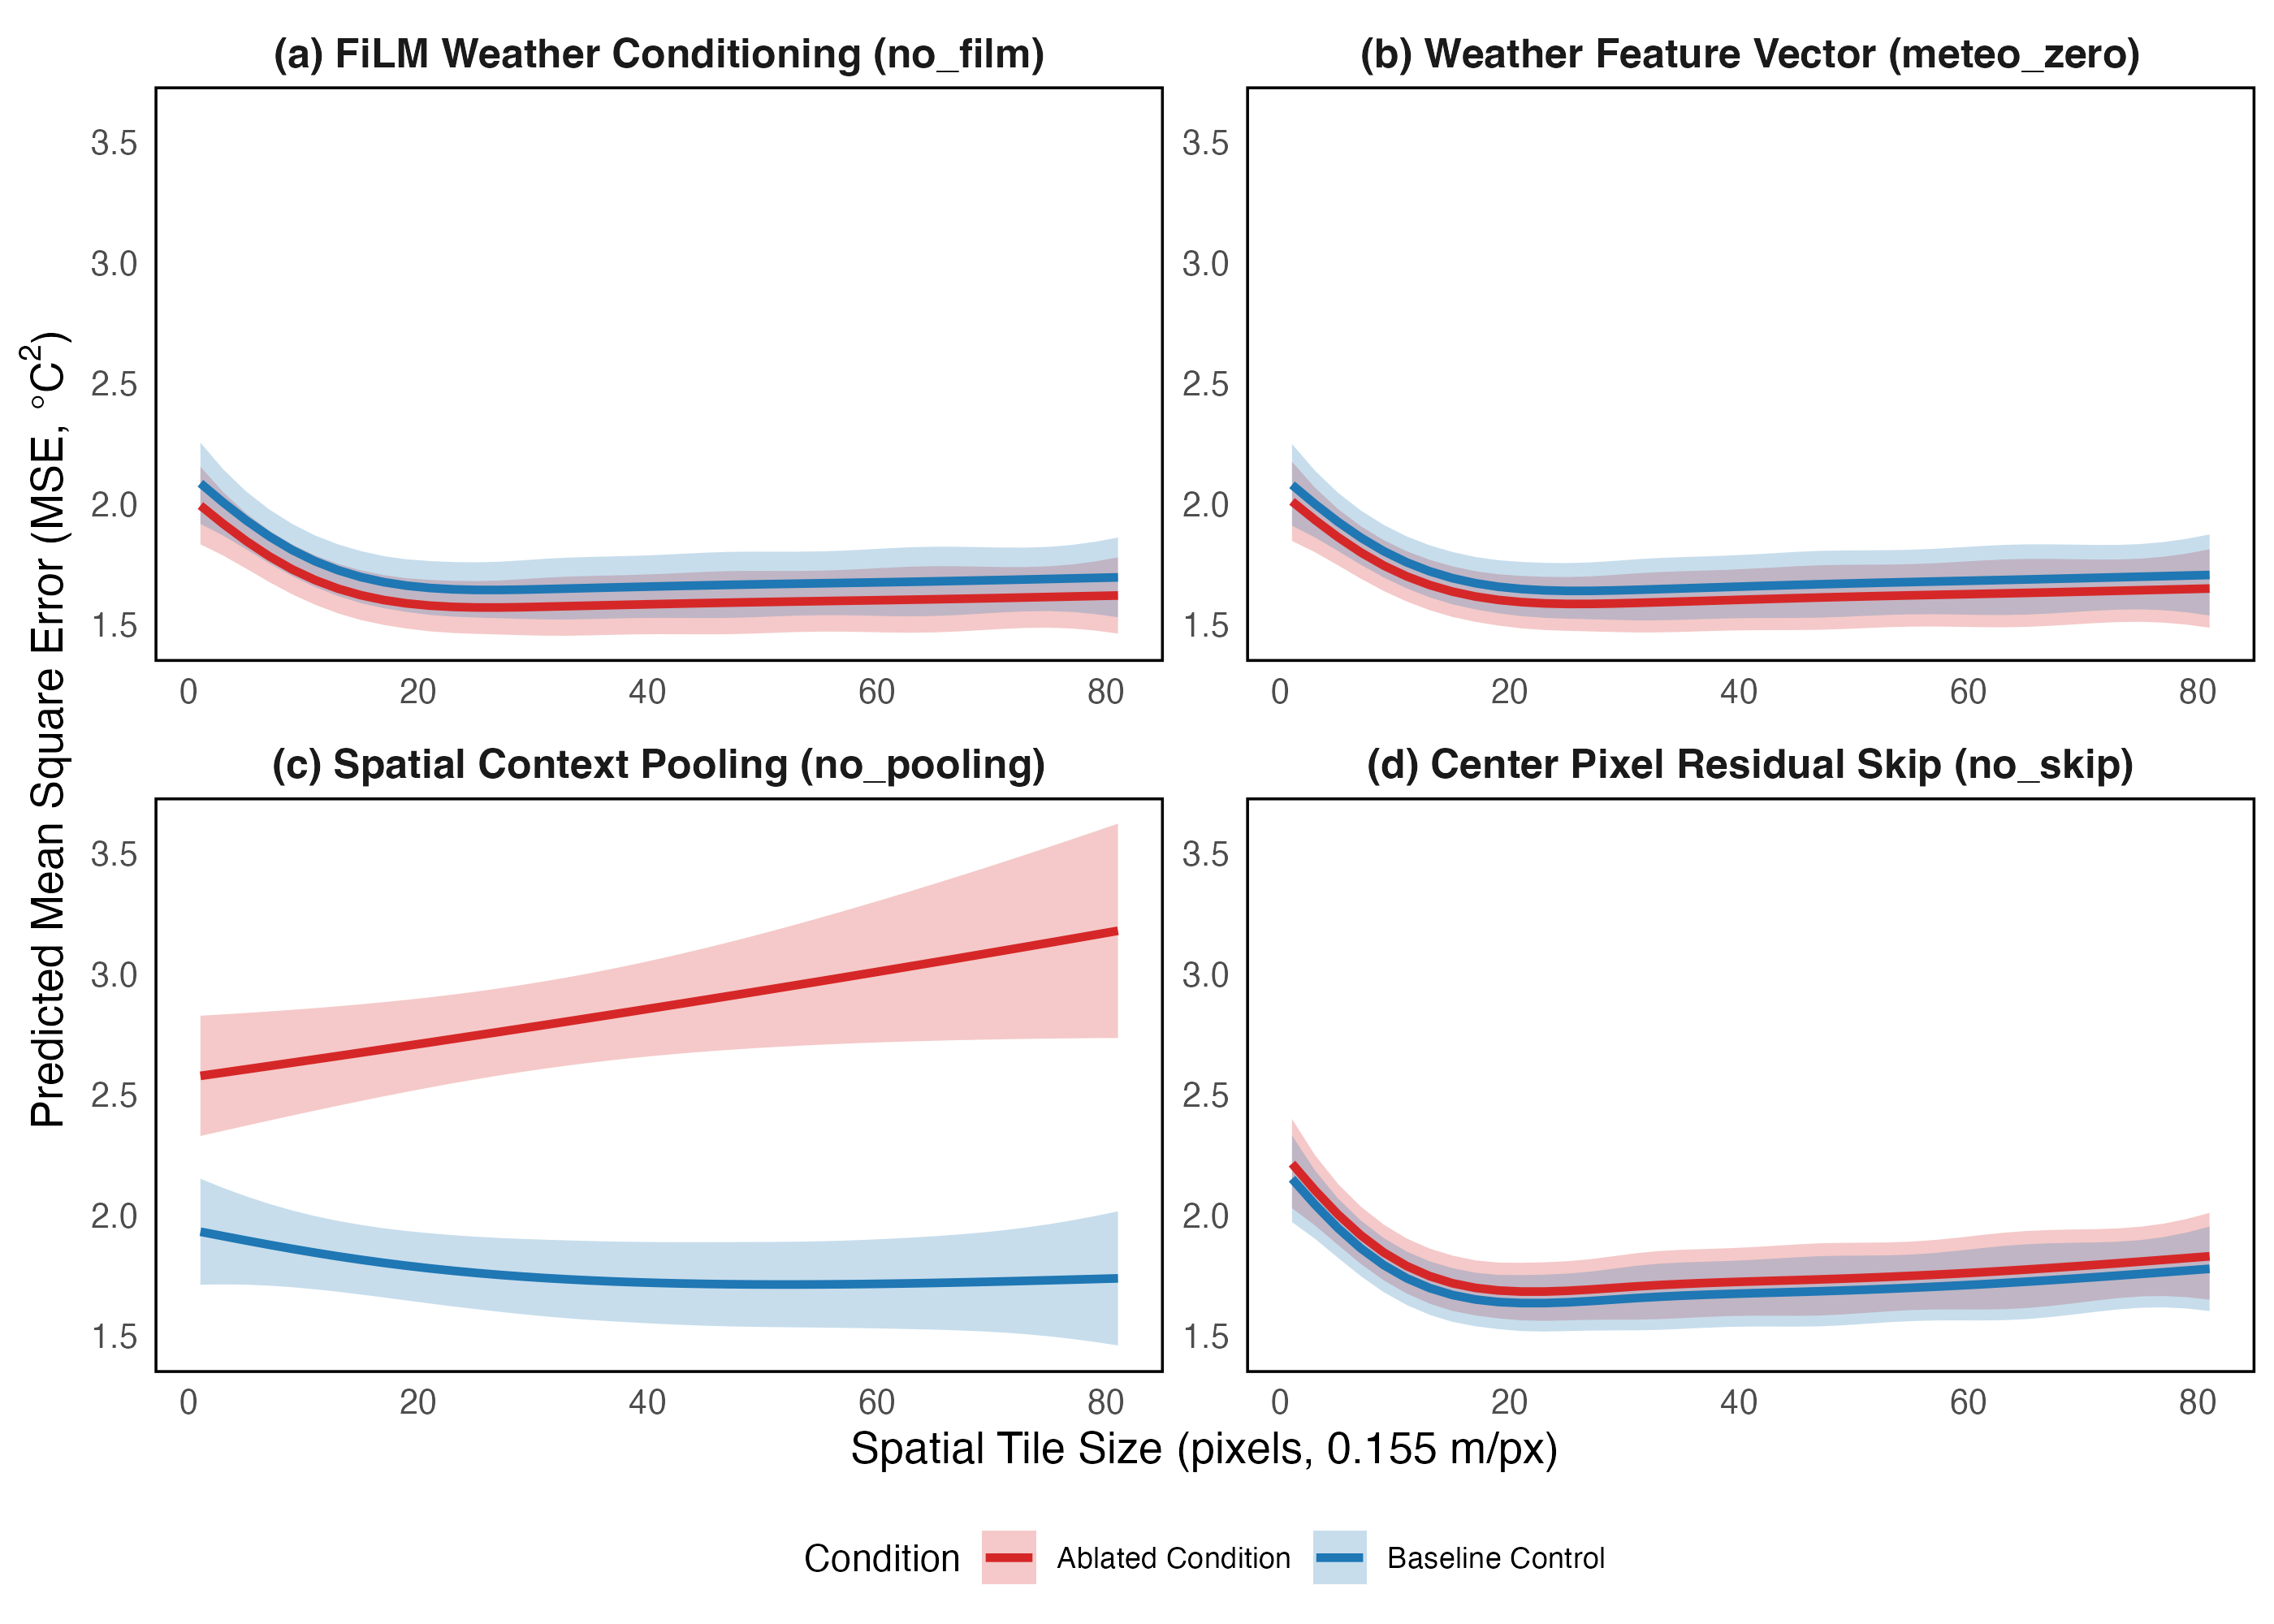
\includegraphics[width=\textwidth]{Figure_final_model_architecture_CI.png}
\caption{Architectural ablation scaling trajectories across spatial tile extents ($1\times1$ to $81\times81$ pixels) evaluated at midday (08:00--16:00). Panels show fitted GAMM marginal trajectories and 95\% confidence intervals (anchored MSE in $^{\circ}\mathrm{C}^2$; i.e., prediction error relative to mean open ground, Eq.~2 in main text) for intact baseline control (blue) versus ablated network configurations (red): (a) removing neighborhood spatial averaging (spatial pooling; $+59.9\%$ MSE surge, $t = 8.33, p < 0.001$), (b) removing dynamic FiLM weather scaling ($-4.4\%$ change, $p = 0.16$), and (c) zeroing all weather features ($-3.3\%$ change, $p = 0.30$). Neighborhood pooling is strictly indispensable for utilizing contextual information beyond a single pixel, whereas macro-meteorological inputs set the whole-scene baseline rather than within-scene microclimatic contrast.}
\label{fig:arch_ablation}
\end{figure}

\section{Mechanistic Physical Microclimate Models and Lateral Heat Exchange}

\subsection{The 1D Surface Energy-Balance Model}

\noindent At each 15~cm pixel ($0.15$~m grid spacing), the baseline model estimates the ground surface (skin) temperature at the moment the drone acquired the thermal image. The surface is an interface with no heat capacity, so it stores no energy: incoming and outgoing fluxes must balance instantaneously. Solar irradiance, atmospheric counter-radiation, and thermal emission from surrounding terrain and vegetation warm the surface. The surface loses heat by emitting longwave radiation, by warming the air through turbulent sensible heat flux, by evaporating water when moisture is available, and by conducting heat into the soil. At each pixel, we solve by Newton--Raphson iteration for the ground skin temperature ($T_g$) at which these gains and losses cancel:
\begin{equation} \label{eq:balance}
S - L - H - E - G = 0\textrm{,}
\end{equation}
\noindent where $S$ is absorbed shortwave radiation, $L$ is net longwave radiation, $H$ is sensible heat flux, $E$ is latent heat flux, and $G$ is soil heat flux, all in $\textrm{W m}^{-2}$. $S$ is positive toward the ground; $L$, $H$, and $E$ are positive away from it, and $G$ is positive into the soil. We describe each term in the order of Eq.~\ref{eq:balance}, followed by the soil initialisation.

The baseline equations follow \citet{Itzkovitch2025}. Where the code used for this study departs from the published implementation, we state the change and its reason in the relevant subsection. None of these baseline corrections involves lateral transport, and all apply equally to the configurations with and without lateral exchange.

\subsubsection{Net Solar Radiation}

\noindent The surface absorbs the fraction of incident sunlight that it does not reflect:
\begin{equation} \label{eq:S}
S = (1 - \alpha) \cdot \textrm{SWR}\textrm{,}
\end{equation}
\noindent where $\alpha$ is the surface shortwave albedo and $\textrm{SWR}$ ($\textrm{W m}^{-2}$) is the total incoming shortwave radiation at the pixel. We computed $\textrm{SWR}$ for every pixel from the drone-derived digital surface model (DSM) with the \textit{r.sun} module of GRASS GIS \citep{GRASS_GIS_software}, which resolves obstruction of the direct beam by relief, rocks, and shrubs. Shaded ground still receives diffuse skylight: 30--80~$\textrm{W m}^{-2}$ across our flights, compared with 200--1000~$\textrm{W m}^{-2}$ on sunlit ground. A separate binary shade raster delineates the microhabitats and reduces wind speed (see Sensible Heat), but it does not set the solar flux in Eq.~\ref{eq:S} to zero.

\subsubsection{Net Longwave Radiation}

\noindent Net longwave flux ($L$) is the thermal emission of the ground minus the longwave radiation it absorbs from the sky and from surrounding terrain and obstacles:
\begin{equation}
L = L_{\textrm{ground}} - L_{\textrm{sky}} - L_{\textrm{obstacles}}\textrm{,}
\end{equation}
\begin{equation}
L_{\textrm{ground}} = \sigma \epsilon_g T_g^4\textrm{,}
\end{equation}
\begin{equation}
L_{\textrm{sky}} = \epsilon_g \, \textrm{SKYV} \left( \sigma \epsilon_{\textrm{sky}} T_{\textrm{ref}}^4 (1-\textrm{CLD}) + \sigma (T_{\textrm{ref}}-2)^4 \, \textrm{CLD} \right)\textrm{,}
\end{equation}
\begin{equation} \label{eq:Lobs}
L_{\textrm{obstacles}} = \epsilon_g (1 - \textrm{SKYV}) \left( \sigma \epsilon_o T_o^4 + (1 - \epsilon_o) L_{\textrm{down}} \right)\textrm{,}
\end{equation}
\noindent where $\sigma = 5.67 \times 10^{-8}~\textrm{W m}^{-2}\textrm{ K}^{-4}$ is the Stefan--Boltzmann constant, $T_{\textrm{ref}}$ (K) is the reference air temperature from the meteorological input, and $T_o$ (K) is the effective temperature of the obstacles that block the sky. The skyview factor ($\textrm{SKYV} \in [0, 1]$) is the fraction of the sky hemisphere not blocked by relief or vegetation, and $\textrm{CLD} \in [0, 1]$ is cloud fraction. Both incoming streams are multiplied by the ground emissivity $\epsilon_g$ because, by Kirchhoff's law, absorptivity equals emissivity. The last term of Eq.~\ref{eq:Lobs} is the downward sky radiation ($L_{\textrm{down}}$) that obstacles reflect toward the pixel. Cloud bases radiate as blackbodies at $T_{\textrm{ref}} - 2~\textrm{K}$. We estimated cloud fraction from the ratio of measured station solar flux to the clear-sky value from \textit{r.sun}, and clear-sky emissivity as $\epsilon_{\textrm{sky}} = 1.72 (e_a / T_{\textrm{ref}})^{1/7}$ \citep{campbell_1998}, with atmospheric vapour pressure $e_a$ in kPa.

Obstacles radiate at the canopy temperature $T_v$ recorded at the weather station ($T_o = T_v$). Over bare terrain (triangular greenness index $TGI < 0.01$ or vegetation height $H_{\textrm{veg}} < 1.0$~m), obstacles take the ground emissivity ($\epsilon_o = \epsilon_g$); over vegetated pixels they take the canopy emissivity ($\epsilon_o = \epsilon_v$). Setting obstacle emission over bare terrain to the mean open-ground temperature of the submap changed shade predictions by only a few tenths of a degree, so we did not adopt it; lateral exchange is thus limited to the single process described in the next section.

\subsubsection{Sensible Heat}

\noindent Sensible heat flux ($H$) is the turbulent transfer of heat between the ground surface and the air above it:
\begin{equation} \label{eq:H}
H = c_{sh} (T_g - T_a) \textrm{,} \qquad c_{sh} = \frac{\rho C_p}{r_{ah}} = \rho C_p C_H u \textrm{,}
\end{equation}
\noindent where $T_a$ (K) is the temperature of the air with which the pixel exchanges heat, $\rho$ is air density ($\textrm{kg m}^{-3}$), $C_p = 1004.64~\textrm{J kg}^{-1}\textrm{ K}^{-1}$ is the specific heat of dry air, and $r_{ah} = (C_H u)^{-1}$ is the aerodynamic resistance ($\textrm{s m}^{-1}$), set by the local wind speed $u$ ($\textrm{m s}^{-1}$) and the dimensionless bulk transfer coefficient $C_H$ \citep{levy_2016b}.

Without lateral exchange, every pixel exchanges heat with the same reference air temperature, $T_a = T_{\textrm{ref}}$ ($T_{AH}$ in the station data). The published code instead used the 2~m air temperature for bare pixels; we now couple all pixels to the same reference level.

Local wind speed $u$ is the station wind $u_{\textrm{station}}$ reduced by drag and sheltering. Over vegetation, canopy drag attenuates it by $\exp(-0.4 \min(2, H_{\textrm{veg}}))$; in shaded pixels, sheltering in the lee of obstacles reduces it by a further $30\%$; and it never falls below $35\%$ of the station wind ($u \ge 0.35\,u_{\textrm{station}}$). The published code set wind to zero in shade, which removes sensible heat exchange altogether and is unrealistic beside a shrub or rock only 1--2~m across; the $30\%$ reduction and the $35\%$ floor replace it. Where vegetation is present ($TGI \ge 0.01$), roughness length scales with canopy height ($z_{0m} = \max(z_{0g}, 0.02 H_{\textrm{veg}})$) and wind speed is bounded by $\max(0.25\,u_{\textrm{station}}, 0.6\,u)$. The local wind speed $u$ sets the sensible heat flux at each pixel, whereas the advected air layer of the lateral model uses the unreduced station wind $u_{\textrm{station}}$ for its relaxation lengths and directional advection calculation (Section~S3.2).

We derived $C_H$ from Monin--Obukhov similarity theory for the surface layer \citep{brutsaert_1982, arya_1988}. The roughness length $z_0$ measures how strongly surface obstacles absorb momentum from the wind. We raised it from the $0.01$~m of smooth bare soil in the published model to $0.03$~m, which represents the gravel, stones, and dwarf shrubs of the Zeelim site, and used equal roughness lengths for momentum and heat ($z_{0h} = z_{0m}$). Atmospheric stability modulates $C_H$ strongly: when the ground is hotter than the air ($T_g > T_a$), buoyant plumes enhance mixing; when it is cooler ($T_g < T_a$), stable stratification damps it. Under neutral stability ($T_g = T_a$), exchange depends only on roughness:
\begin{equation} \label{eq:neutral}
C_{H,\textrm{neutral}} = \frac{\kappa^2}{\left[ \ln \left( \frac{z + z_0}{z_0} \right) \right]^2}\textrm{,}
\end{equation}
\noindent where $\kappa = 0.40$ is the von K\'arm\'an constant and $z = 2.0$~m is the reference height. This stability correction lies at the heart of the shadow problem: standard similarity theory treats a shaded patch as an isolated cold surface and therefore suppresses its heat exchange.

\subsubsection{Latent Heat Flux}

\noindent Latent heat flux ($E$) is the heat removed by evaporation:
\begin{equation}
E = c_{ev} (e_s(T_g) RH_{\textrm{soil}} - e_a)\textrm{,} \qquad c_{ev} = \frac{\rho C_p}{\gamma (r_{aw} + r_s)}\textrm{,}
\end{equation}
\noindent where $e_s(T_g)$ is the saturation vapour pressure at ground temperature (Pa), $e_a$ is atmospheric vapour pressure (Pa), $\gamma$ is the psychrometric constant ($\textrm{Pa K}^{-1}$), $r_{aw} = r_{ah}$ is the aerodynamic resistance to water vapour, and $r_s$ is the soil surface resistance ($\textrm{s m}^{-1}$). The relative humidity in the surface soil pores ($RH_{\textrm{soil}}$) follows from the matric suction head $\psi = -\psi_{\textrm{sat}} (\theta_1 / \theta_{\textrm{sat}})^{-b}$ through the Kelvin relation \citep{niu_2011}. At our hyper-arid site, the topsoil stays desiccated throughout late summer ($\theta_1 < 0.01~\textrm{m}^3\textrm{ m}^{-3}$), surface resistance reaches $r_s = 10^6~\textrm{s m}^{-1}$, and latent heat flux is effectively zero. Evaporation cools the surface substantially only after spring rain.

\subsubsection{Heat Flux in Soil}

\noindent Soil heat flux ($G$) conducts energy from the surface into the soil:
\begin{equation} \label{eq:G}
G = c_{gh} (T_g - T_{\textrm{soil},1})\textrm{,} \qquad c_{gh} = \frac{k}{\Delta z_1 / 2} = \frac{2k}{\Delta z_1}\textrm{,}
\end{equation}
\noindent where $T_{\textrm{soil},1}$ (K) is the temperature at the midpoint of the top soil layer, $k$ is thermal conductivity ($\textrm{W m}^{-1}\textrm{ K}^{-1}$), and $\Delta z_1 = 0.03$~m is the layer thickness. Heat therefore travels the half-layer distance $\Delta z_1 / 2 = 1.5$~cm between the surface and the layer midpoint. The published code used a fixed $10$~cm spacing ($c_{gh} = 2k/0.1$), which does not correspond to the model's 3~cm layers; using the true half-layer distance triples the thermal coupling between surface and soil. The soil column comprises 66 layers of $3$~cm each, reaching $1.98$~m depth. Thermal conductivity and volumetric heat capacity follow the Noah-MP parameterisations \citep{niu_2011} for sandy loam / loamy sand (soil type 4: quartz fraction $0.25$, porosity $\theta_{\textrm{sat}} = 0.476$, saturated suction $\psi_{\textrm{sat}} = 0.759$~m, Campbell exponent $b = 5.33$).

\subsubsection{Soil Profile Initialisation via 24-Hour Spin-Up}

\noindent Eq.~\ref{eq:G} shows that the skin temperature depends on the temperature of the soil directly beneath it, so the soil must start from a realistic profile. The published model prescribed a single daily profile from sparse meteorological observations. This profile underestimates afternoon temperatures in the shallow soil by $15\text{--}20$~K and so drains more than $100~\textrm{W m}^{-2}$ from the surface. We replaced it with a spin-up: for the 24 hours preceding each flight, we ran a single bare-soil column through the model's full equations at a $300$~s time step, forced by hourly ERA5-Land reanalysis \citep{ERA5} bias-adjusted to the on-site station (with reanalysis downward longwave radiation supplying the atmospheric irradiance). The spin-up requires no calibration, and one 24-hour pass suffices: a second pass shifts the flight-time surface temperature by $<0.05$~K and the topsoil by $<0.3$~K, and changes only deep layers ($>20$~cm) whose thermal response time exceeds a day.

%The spun-up profile initialises every pixel of the map. We first diagnose $T_g$ in balance with this profile without advancing the soil, then advance the map by two $300$~s time steps ($10$~minutes) of vertical heat conduction, re-diagnosing $T_g$ after each step so that the final skin temperature is in equilibrium with the topsoil. The conduction solver drives the soil update directly with the diagnosed surface flux $G$ and is written in conservative tridiagonal form. This form corrects two errors in the published Thomas solver (\texttt{ROSR12}): an input coefficient that was overwritten during the solve, and a missing heat-storage term.

%The 66-layer column resolves the thermal memory of the soil explicitly. % \textit{microclimf}, which is described in Section~S3.3, instead approximates ground heat flux from the departure of the instantaneous surface temperature from its running daily mean \citep{maclean_2026}.

\subsubsection{The Model Simulation: The Uncoupled Column Assumption}

\noindent In the 1D model described so far, every pixel is solved in isolation. Terrain, solar irradiance, and skyview vary among pixels, but nothing in Eq.~\ref{eq:balance} lets neighbouring patches interact: a shaded pixel exchanges heat with the atmosphere as if it lay on an infinite shaded plain. This assumption suits broad, uniform landscapes but fails for a 1--2~m shadow surrounded by sunlit ground $10\degree$C hotter. The next section describes how we let neighbouring patches exchange heat.

\subsection{Coupled 2D Lateral Heat Exchange Between Patches}

\noindent The main text motivates the coupled lateral process and illustrates it conceptually (Main Text Fig.~4). Here we give its formulation. The process acts on the two factors of the sensible heat term (Eq.~\ref{eq:H}): the temperature of the air with which the ground exchanges heat, which we represent by an advected near-surface air layer, and the exchange coefficient, which is prevented from dropping artificially over shaded ground by a neutral-stability floor. The two terms operate together.

\subsubsection{Advected Near-Surface Air Layer}

\noindent The first term sets the temperature of the air. In the 1D model, every pixel exchanges sensible heat with the same reference air temperature recorded at the weather station ($T_{\textrm{ref}}$, at 2~m height; Eq.~\ref{eq:H}). However, air blowing into a shadow has just crossed hot sunlit ground and arrives substantially warmer than $T_{\textrm{ref}}$, especially near the upwind edge.

To represent this, we track the temperature $T_{\textrm{air}}$ (K) of a thin near-surface air layer as the wind carries it across the terrain. Turbulent heat exchange with the surface drives the layer temperature toward the local skin temperature $T_g$, while vertical mixing with the undisturbed background air above relaxes it back toward $T_{\textrm{ref}}$. Along the wind direction, with distance $s$, this balance reads:
\begin{equation} \label{eq:advect}
u_{\textrm{station}} \frac{d T_{\textrm{air}}}{d s} = \frac{T_g - T_{\textrm{air}}}{\tau_g} - \frac{T_{\textrm{air}} - T_{\textrm{ref}}}{\tau_e}\textrm{,}
\end{equation}
\noindent where $u_{\textrm{station}}$ is the station wind speed, which we apply uniformly over the map, and $\tau_g$ and $\tau_e$ (s) are the relaxation time scales toward the ground and the background air. Multiplying these time scales by wind speed converts them into relaxation lengths ($L_g = u_{\textrm{station}} \tau_g$ and $L_e = u_{\textrm{station}} \tau_e$), which represent the horizontal distances over which the moving air temperature adjusts toward the temperature of the ground beneath it ($L_g$) and the undisturbed air above ($L_e$). We set $L_g = 1.0$~m and $L_e = 2.5$~m at $u_{\textrm{station}} = 2~\textrm{m s}^{-1}$ (Table~\ref{table:lateralparam}) and scaled both by $f = \textrm{clamp}(u_{\textrm{station}} / 2.0, 0.5, 2.0)$, so that they shorten in light winds and lengthen in strong winds. The sensible heat flux itself (Eq.~\ref{eq:H}) uses the local wind speed.

Over uniform ground, Eq.~\ref{eq:advect} reaches a steady state:
\begin{equation} \label{eq:local}
T_{\textrm{air,uniform}} = \frac{L_e T_g + L_g T_{\textrm{ref}}}{L_g + L_e}\textrm{,}
\end{equation}
\noindent a weighted average dominated by the ground temperature because $L_g < L_e$. Across an abrupt step in ground temperature, such as a shadow margin, the layer approaches this steady state over a relaxation distance $L_g L_e / (L_g + L_e) \approx 0.7$~m at $2~\textrm{m s}^{-1}$ ($0.4\text{--}1.4$~m across our flights). This distance determines how far the wind carries heat from sunlit ground into a shadow before the air cools. As this warm air crosses the boundary, it transfers sensible heat to the shaded ground, creating the warm margins observed along shadow edges \citep{mott_2013, essery_2006}.

We solved Eq.~\ref{eq:advect} using an implicit upwind finite-difference scheme along the wind direction:
\begin{equation} \label{eq:march}
T_{\textrm{air}}(s + \Delta s) = \frac{T_{\textrm{air}}(s) + a \, T_g + b \, T_{\textrm{ref}}}{1 + a + b}\textrm{,} \qquad a = \frac{\Delta s}{L_g}\textrm{,} \quad b = \frac{\Delta s}{L_e}\textrm{,}
\end{equation}
\noindent where $\Delta s$ is the pixel step along the wind. The spatial integration begins at the upwind domain boundary using Eq.~\ref{eq:local}. When the wind is oblique to the grid, the upwind point falls between grid positions, and we interpolate linearly between the two adjacent upwind cells. Wind direction is the 10-min vector average recorded by the weather station at flight time (the latest record at or before the flight; Table~\ref{table:winddir}), the same record that supplies the wind speed.

We couple the advected air to the surface energy balance through its departure from the local steady state:
\begin{equation} \label{eq:anomaly}
T_a = T_{\textrm{ref}} + \phi \left( T_{\textrm{air}} - T_{\textrm{air,uniform}} \right)\textrm{.}
\end{equation}
\noindent This $T_a$ enters the sensible heat term (Eq.~\ref{eq:H}); longwave fluxes still use $T_{\textrm{ref}}$. Because the temperature anomaly ($T_{\textrm{air}} - T_{\textrm{air,uniform}}$) equals zero over uniform terrain, this lateral correction leaves predictions across open ground unchanged and acts only across thermal boundaries. The scaling factor $\phi = 3.0$ accounts for the vertical height of the advected layer: because isolated shadows are only 1--2~m across, the advected thermal boundary layer is shallow and confined to the roughness sublayer within $\sim 10\text{--}15$~cm of the surface. In a logarithmic surface layer ($z_0 = 0.03$~m), aerodynamic resistance to this shallow height is roughly one third of the resistance to the 2~m reference height ($\ln(2.0/0.03) / \ln(0.12/0.03) \approx 4.2 / 1.4 \approx 3$). Scaling the near-surface temperature departure by $\phi = 3.0$ therefore ensures that the 2~m bulk sensible heat formulation (Eq.~\ref{eq:H}) transfers the correct heat flux to the ground, consistent with our calibration against observed shadow-edge transects (Table~\ref{table:lateralparam}).

During each $300$~s time step, the air anomaly and ground skin temperature ($T_g$) are brought to mutual consistency through a 20-pass iterative coupling. At the start of the step, the upwind advection scheme (Eq.~\ref{eq:march}) sweeps across the terrain along the wind direction to compute the initial near-surface air temperature $T_a$ (Eq.~\ref{eq:anomaly}) from the current $T_g$ map. In each subsequent iteration:
(1) ground skin temperature $T_g$ is re-diagnosed at each pixel by solving the surface energy balance (Eq.~\ref{eq:balance}) using the calculated air temperature $T_a$ in the sensible heat flux (with the subsurface soil column held fixed);
(2) the upwind advection scheme (Eq.~\ref{eq:march}) sweeps across this updated $T_g$ map to compute the new advected air temperature anomaly; and
(3) the effective air temperature $T_a$ is updated using an under-relaxation factor of $0.25$ (applying 25\% of the newly computed anomaly change and 75\% of the previous value, bounded to $\pm 20$~K) to prevent numerical oscillations across sharp shadow margins.
This damped iteration converges smoothly to a stable equilibrium, yielding consistent temperatures across successive time steps (Fig.~\ref{fig:lateral_cells}).

\subsubsection{Turbulent Exchange Floor Near a Shadow}

\noindent The second term sets the rate of exchange with that air. Monin--Obukhov similarity theory assumes a horizontally homogeneous surface and suppresses heat exchange when the ground is cooler than the air, because stable stratification resists vertical mixing. This assumption holds over extensive cold surfaces such as lakes or snowfields, but fails for a 1--2~m shadow. Air entering a narrow shadow has been intensely mixed by convection over the surrounding sunlit ground, and this turbulence does not decay over the 1--2 seconds required to traverse the shadow. However, an uncoupled 1D model evaluates stability based solely on the local surface temperature, artificially suppressing turbulent heat exchange to approximately one third of the open-ground rate.

We prevented this unphysical suppression by imposing a neutral-stability floor on the bulk transfer coefficient $C_H$ (Eq.~\ref{eq:neutral}):
\begin{equation} \label{eq:floor}
C_H = \max \left( C_{H,\textrm{stability}}, \; C_{H,\textrm{neutral}} \right)\textrm{,}
\end{equation}
\noindent where $C_{H,\textrm{stability}}$ is the Monin--Obukhov value. Equation~\ref{eq:floor} reflects the condition that turbulent mixing over a small shaded patch is maintained by turbulent kinetic energy advected from the surrounding landscape. Across heterogeneous surfaces, advection of turbulence from surrounding heated or rough terrain prevents boundary-layer decoupling, maintaining near-neutral atmospheric exchange over isolated cool patches \citep{helgason_2012}. Setting $C_H$ to its neutral value restores this background turbulent mixing over shaded ground. We apply the same floor to the momentum transfer coefficient $C_M$, whose neutral value equals $C_{H,\textrm{neutral}}$ because $z_{0h} = z_{0m}$; $C_M$ sets the friction velocity in the stability calculation.

These two lateral mechanisms are closely coupled: without the turbulent floor (Eq.~\ref{eq:floor}), stable stratification decouples the surface layer and prevents the warm advected air from transferring heat downward; without the advected air layer (Eq.~\ref{eq:anomaly}), enhanced mixing merely couples the shaded ground more tightly to the cooler background air ($T_{\textrm{ref}}$) \citep{mott_2013}. Across held-out test blocks from all 10 evaluation flights, this coupled lateral formulation substantially reduced shaded ground prediction error and resolved the severe shade-cooling bias (Table~\ref{tab:comparison_summary}).

\begin{figure}[!ht]
\centering
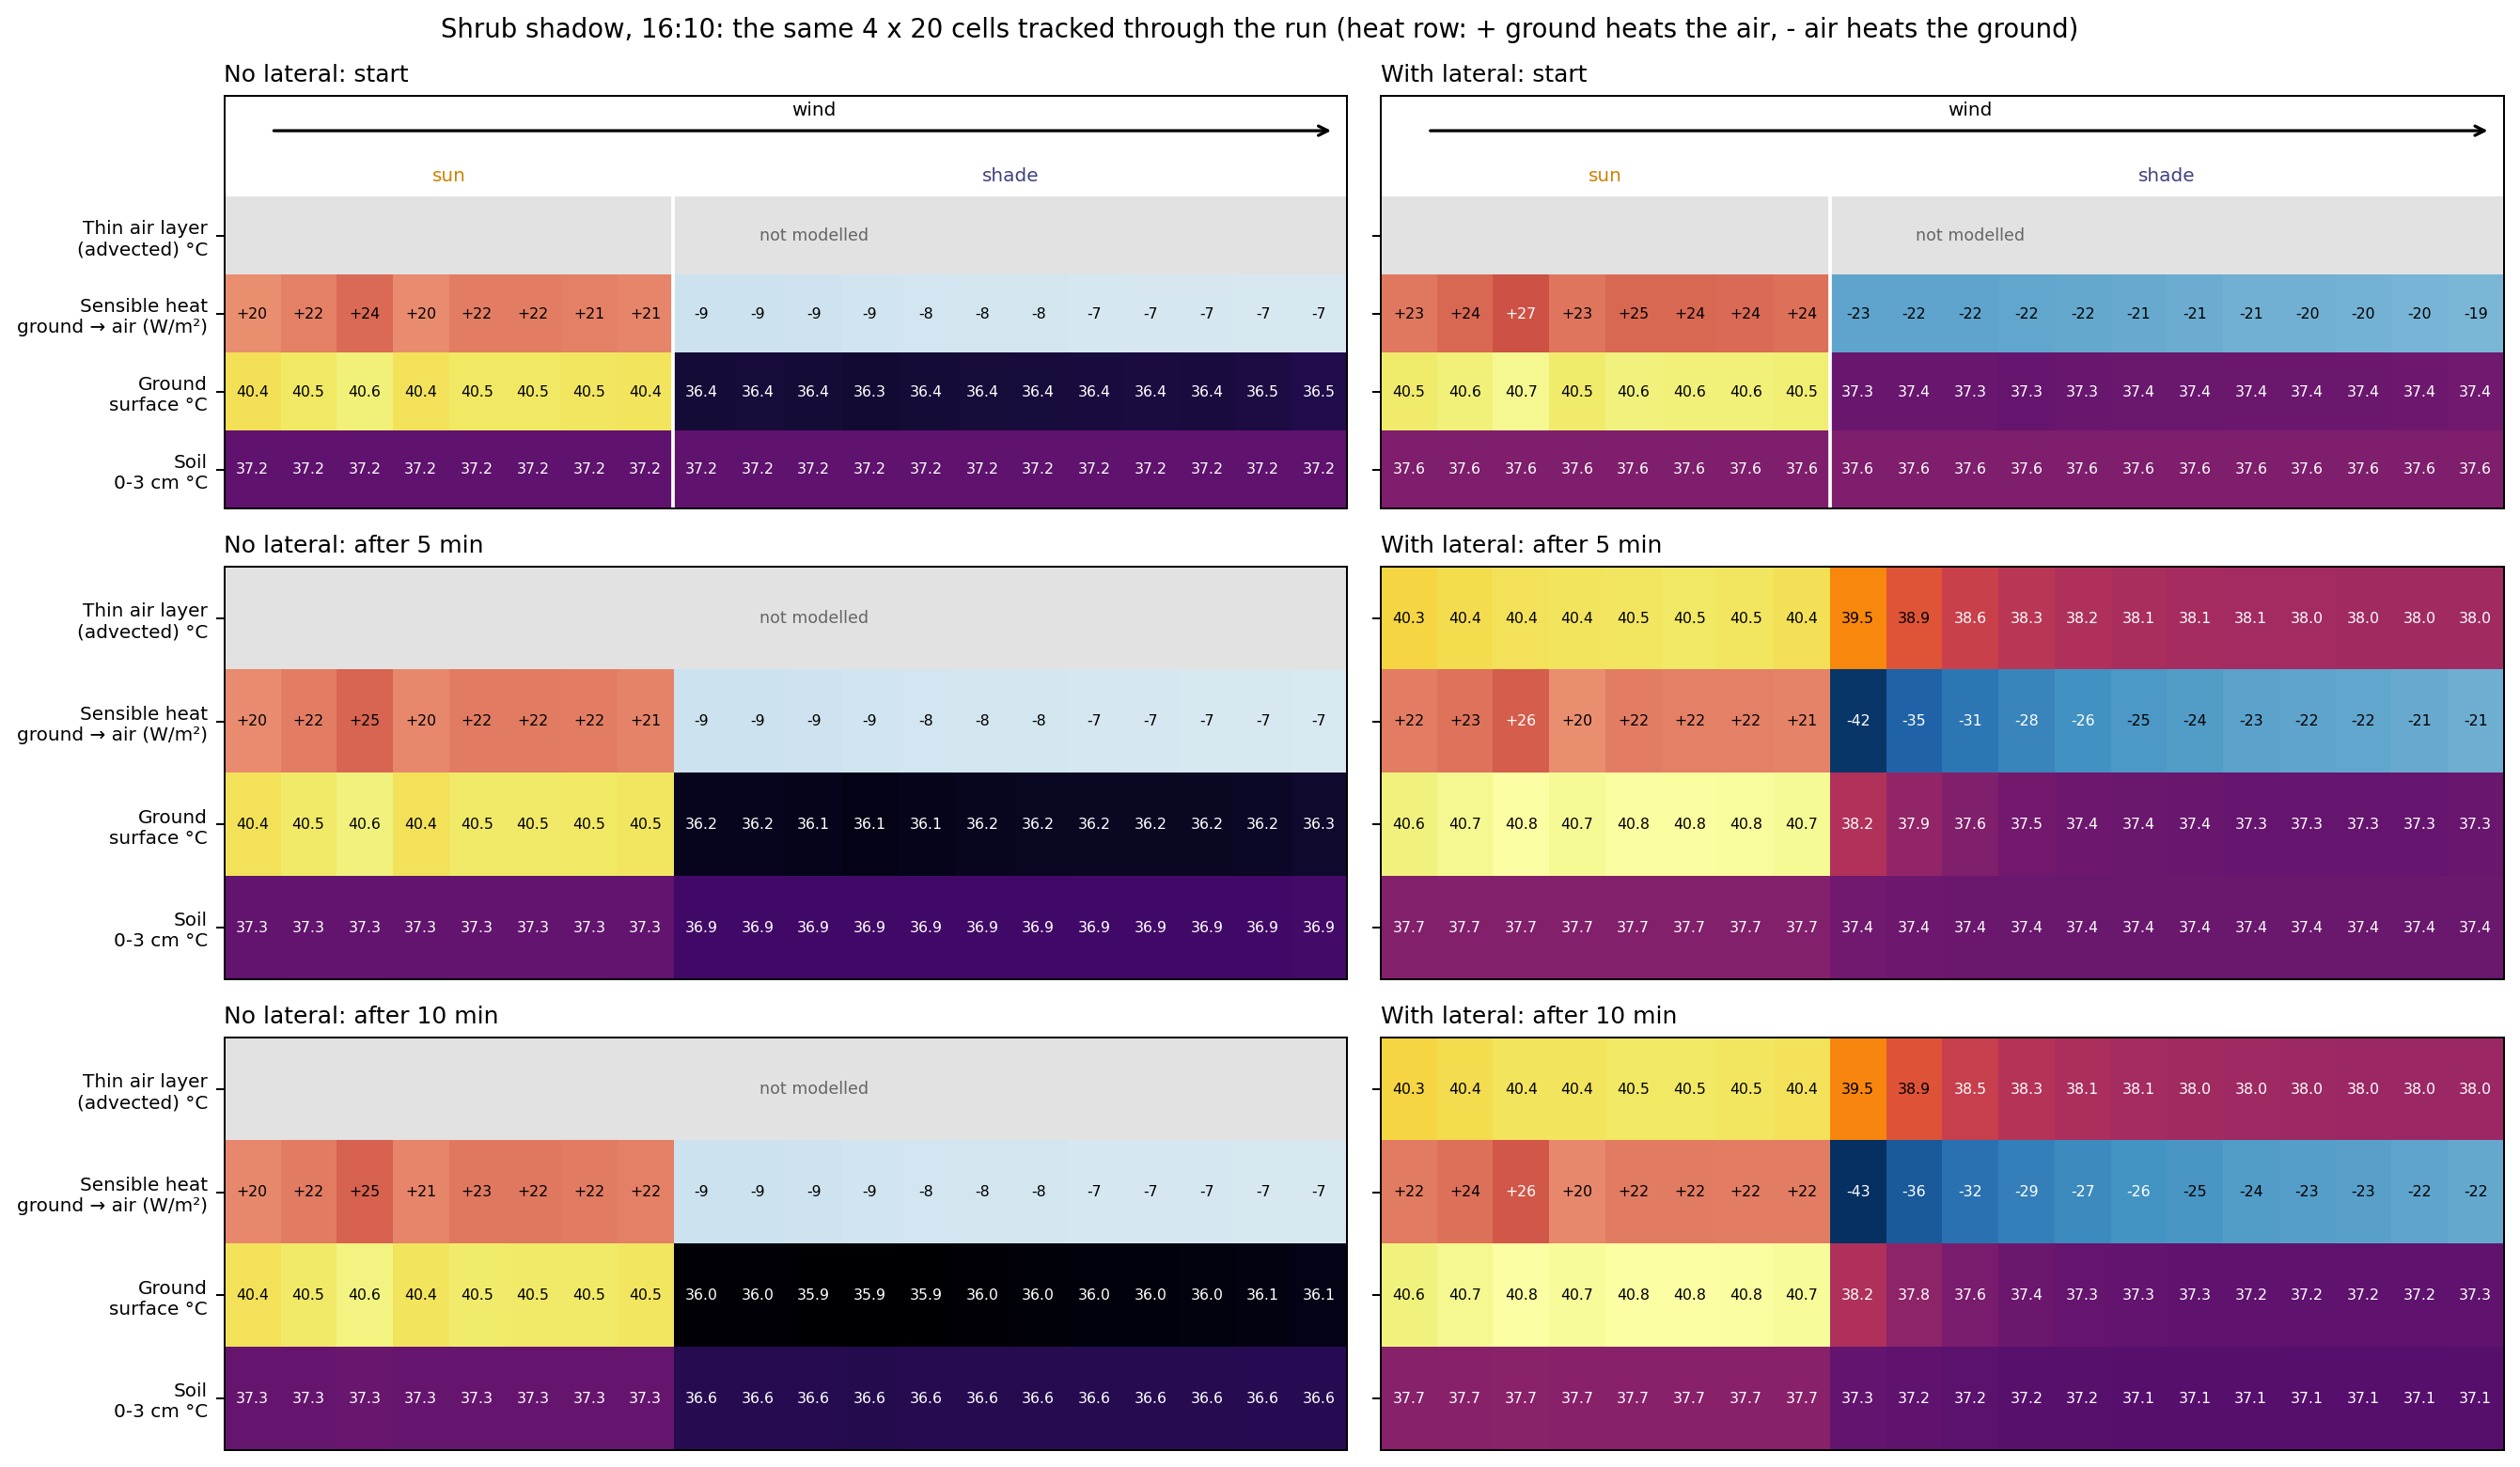
\includegraphics[width=\textwidth]{Figure_lateral_cells_tracked_1610.png}
\caption{Lateral heat exchange at a shadow margin, followed through the model run. Twenty adjacent pixels (3.1~m) along the wind (from $350^\circ$, the station direction of the flight) across the edge of a shrub shadow (flight of 16:10 on 23 September 2019), eight sunlit and twelve shaded, at the start of the run, after the first and after the second $300$~s time step, without (left) and with (right) lateral exchange. Rows show the advected near-surface air layer (\degree C; computed only with lateral exchange), the sensible heat flux from ground to air (W~m$^{-2}$; positive values heat the air, negative values heat the ground), the ground skin temperature (\degree C) and the temperature of the first 3~cm of soil (\degree C). Without lateral exchange the shaded ground receives less than 10~W~m$^{-2}$ from the air and cools slowly as its soil column, initialised as open sand, loses heat. With lateral exchange the air entering the shade is still above 39~\degree C and cools to 38~\degree C within a metre, the shaded ground receives 20--45~W~m$^{-2}$, most within the first metre, and warms by 1--2~\degree C, while the soil beneath changes by less than 1~\degree C. The two time steps yield consistent equilibrium values, as expected from the converged iterative solution (Section~S3.2).}
\label{fig:lateral_cells}
\end{figure}

% \subsection{Implementation and Arid Configuration of \textit{microclimf}}
% 
% \noindent We ran \textit{microclimf} \citep{maclean_2026}, which is described in the main text, across the held-out 50$\times$50~m test blocks for all 10 evaluation flights at the native 15~cm resolution.
% 
% \subsubsection{Physical Adaptations and Numerical Corrections for Hyper-Arid Terrain}
% 
% \noindent The default \textit{microclimf} settings were developed for temperate landscapes above sea level and produced severe artefacts in the below-sea-level Dead Sea basin. We made five adaptations, without altering the package's core equations:
% \begin{enumerate}[nosep]
%     \item \textit{Edge-clamping at negative elevation (Dead Sea horizon artefact).} The \textit{microclimf} routines \texttt{.horizon} and \texttt{.windsheltera} pad the DEM with a 100-pixel buffer at $0.0$~m elevation. Because Zeelim lies $240$--$261$~m below sea level, this padding erected an artificial $250$~m cliff around every submap, which cast 10 concentric shadow rings inward. We instead padded by edge-clamping, replicating the perimeter elevations outward to preserve the true terrain slopes.
%     \item \textit{On-site meteorological calibration and solar blending.} Raw ERA5-Land reanalysis performs poorly in desert basins: it underestimated morning insolation by up to 90\%, overestimated midday solar flux by 34\%, and was 2--3.6\degree C too cold. We harmonised the 24 h ERA5-Land sequence with the on-site tower at the flight hour: we scaled downward solar flux to the station pyranometer across a Gaussian temporal window ($\sigma = 2.0$~h), shifted air temperature by the station offset, scaled wind speed to the anemometer, calibrated relative humidity and pressure to measured values, and partitioned diffuse radiation hourly.
%     \item \textit{Arid soil moisture and albedo.} The temperate defaults ($\theta = 0.35~\textrm{m}^3\textrm{ m}^{-3}$, $\alpha = 0.15$) produced unphysical latent heat fluxes over dry sand ($>400~\textrm{W m}^{-2}$). For dry summer flights, we set volumetric soil moisture to $\theta = 0.08~\textrm{m}^3\textrm{ m}^{-3}$ (matching the top 10~cm probes), shortwave albedo to $\alpha = 0.20$, and deep soil temperature to $30.44\degree$C (matching the 100~cm probe). For the spring flight (12 April 2021), when annual plants were active, we set $\theta = 0.18~\textrm{m}^3\textrm{ m}^{-3}$, $\textrm{PAI} = 1.2$, and $g_{s\max} = 0.33~\textrm{mol m}^{-2}\textrm{ s}^{-1}$.
%     \item \textit{Solid obstacles rather than transpiring canopy.} By default, \textit{microclimf} treats shading obstacles as transpiring foliage ($g_{s\max} = 0.33~\textrm{mol m}^{-2}\textrm{ s}^{-1}$), which drove shaded ground beside rocks down to dewpoint temperatures ($\sim 17\degree$C). For dry flights, we set stomatal conductance and plant area index to zero ($g_{s\max} = 0$, $\textrm{PAI} = 0$), so that shade acts only as geometric obstruction on the DSM.
%     \item \textit{Time zone alignment.} We standardised timestamps to Israel Standard Time (IST = UTC+2 year-round), which removed an initial 1--2 hour mismatch in solar angle.
% \end{enumerate}

%TC:endignore


\newpage

\begin{table}[h]
\centering
\begin{tabular}{|l|l|l|}
\hline
Set & Date & Time \\ \hline
Train & 18.9.19 & 09:00, 12:00, 14:00, 15:00, 17:20 \\ \hline
 & 29.5.19 & 08:30, 16:50, 17:30 \\ \hline
 & 30.1.20 & 09:20, 09:50, 10:50, 12:00, 13:00, 13:50, 14:49, 15:23 \\ \hline
 & 30.5.19 & 06:00, 06:30 \\ \hline
 & 7.11.19 & 10:30, 11:00, 13:10, 15:50, 16:40 \\ \hline
Test & 12.04.21 & 11:18 \\ \hline
 & 23.09.19 & 06:10, 07:00, 08:00, 14:10, 15:10, 16:10 \\ \hline
 & 31.05.21 & 15:16, 17:12, 18:05 \\ \hline
\end{tabular}
\caption{Dates and times of the drone flight surveys. A total of 33 flights were conducted on different dates to build the dataset. Data from these flights were geographically partitioned via 50$\times$50~m spatial blocking to train and test the spatially aware deep learning and physical microclimate models.}
\label{table:flights}
\end{table}

\newpage

\begin{table}[h]
\centering
\adjustbox{max width=\textwidth}{%
\small
\begin{tabular}{|c|p{7.5cm}|c|c|c|}
\hline
\textbf{Model} & \textbf{Formula Specification} & \textbf{Est.~df} & \textbf{AIC} & $\boldsymbol{\Delta}$\textbf{AIC} \\ \hline
\textbf{M4} & \textbf{\texttt{s(size, by=time\_class) + microhabitat * time\_class}} & \textbf{20.2} & \textbf{2255.9} & \textbf{0.0} \\ \hline
M3 & \texttt{s(size, by=time\_class) + microhabitat} & 18.4 & 2270.8 & 14.9 \\ \hline
M5 & \texttt{s(size, by=time\_class) + microhabitat + time\_class} & 18.2 & 2270.9 & 15.0 \\ \hline
M7 & \texttt{s(size, by=microhabitat\_time)} & 19.9 & 2657.7 & 401.8 \\ \hline
M6 & \texttt{s(size, by=time\_class) + s(size, by=microhabitat)} & 19.5 & 2659.3 & 403.3 \\ \hline
M2 & \texttt{s(size, by=time\_class)} & 17.0 & 2667.6 & 411.7 \\ \hline
M1 & \texttt{s(size) + s(size, by=morning) + s(size, by=evening)} & 19.6 & 2683.0 & 427.1 \\ \hline
M8 & \texttt{s(size) + time\_class} & 13.2 & 2688.1 & 432.2 \\ \hline
M9 & \texttt{Linear(size * time\_class)} & 13.0 & 2703.3 & 447.4 \\ \hline
\end{tabular}%
}
\caption{Model selection results across candidate Generalized Additive Mixed-Effects Models (GAMMs) evaluating the scaling of prediction error (anchored MSE; i.e., prediction error relative to mean open ground, Eq.~2 in main text) with spatial tile size across diurnal dayparts and microhabitats. All models include flight identity as a random intercept (\texttt{s(flight, bs="re")}) and assume a Gamma error distribution with a log link function. Model M4, which incorporates daypart-specific non-linear spatial smooths and a microhabitat $\times$ daypart interaction, was decisively selected by Akaike's Information Criterion ($\Delta\text{AIC} = 0.0$).}
\label{table:gamm_aic}
\end{table}

\newpage

\begin{table}[h]
\centering
\adjustbox{max width=\textwidth}{%
\small
\begin{tabular}{|l|c|c|c|c|c|}
\hline
\textbf{Ablated Layer / Condition} & \textbf{Ratio ($\boldsymbol{\frac{\text{Ablated}}{\text{Baseline}}}$)} & \textbf{\% $\boldsymbol{\Delta}$MSE} & \textbf{SE} & $\boldsymbol{t}$\textbf{-ratio} & $\boldsymbol{p}$\textbf{-value} \\ \hline
\texttt{real\_solar} & 1.840 & $+84.0\%$ & 0.082 & 13.60 & $<0.001$ \\ \hline
\texttt{skyview} & 1.288 & $+28.8\%$ & 0.053 & 6.15 & $<0.001$ \\ \hline
\texttt{shade} & 1.212 & $+21.2\%$ & 0.055 & 4.25 & $<0.001$ \\ \hline
\texttt{height} & 1.133 & $+13.3\%$ & 0.039 & 3.59 & $<0.001$ \\ \hline
\texttt{TGI} & 1.093 & $+9.3\%$ & 0.040 & 2.40 & $0.017$ \\ \hline
\texttt{no\_pooling} & 1.599 & $+59.9\%$ & 0.090 & 8.33 & $<0.001$ \\ \hline
\texttt{no\_film} & 0.956 & $-4.4\%$ & 0.031 & $-1.41$ & $0.160$ \\ \hline
\texttt{meteo\_zero} & 0.967 & $-3.3\%$ & 0.031 & $-1.03$ & $0.302$ \\ \hline
\end{tabular}%
}
\caption{Pairwise Generalized Additive Mixed-Effects Model (GAMM) contrasts evaluating the effect of physical feature and architectural ablations at midday (08:00--16:00) on anchored prediction error (MSE; i.e., prediction error relative to mean open ground, Eq.~2 in main text). Models evaluate the response ratio and percentage change in prediction error ($\%\Delta\text{MSE}$) of ablated conditions compared to the intact baseline control across spatial tile sizes using empirical marginal response estimates via \textit{emmeans} ($N = 17{,}550$ submap evaluations). Architectural ablations test spatial pooling and weather conditioning: \texttt{no\_pooling} disables neighborhood spatial averaging across the tile, \texttt{no\_film} disables Feature-wise Linear Modulation (FiLM), and \texttt{meteo\_zero} sets all macro-meteorological inputs to zero. Direct solar radiation, skyview exposure, microtopography, and spatial pooling contribute significantly to midday prediction accuracy, whereas macro-meteorological inputs set the whole-scene baseline rather than localized within-scene microclimatic contrast.}
\label{table:ablation_contrasts}
\end{table}

\newpage

\begin{table}[ht]
\centering
\begingroup\small\renewcommand{\baselinestretch}{1.0}\selectfont
\renewcommand{\arraystretch}{1.15}
\begin{tabular}{ |p{2.6cm}||p{2.4cm}|p{9.5cm}| }
 \hline
 Symbol & Value & Description \\
 \hline
 $z_0$ & 0.03 m & Roughness length of the ground surface, raised from the 0.01 m of smooth bare soil to a value representative of gravel, stones and sparse shrubs. Common to both configurations \\
 \hline
 $L_g$ & 1.0 m & Distance the near-surface air must travel before it responds to the temperature of the ground beneath it, at a wind speed of 2 m s$^{-1}$ \\
 \hline
 $L_e$ & 2.5 m & Distance over which the near-surface air is pulled back towards the undisturbed air above, at a wind speed of 2 m s$^{-1}$ \\
 \hline
 $\frac{L_g L_e}{L_g + L_e}$ & 0.7 m & Resulting distance over which the air carries the warmth of sunlit ground into a shadow, at a wind speed of 2 m s$^{-1}$ (0.4--1.4 m over our flights) \\
 \hline
 $\phi$ & 3 & Ratio between the influence on the surface of the thin near-surface air layer and that of the air at the 2 m reference height \\
 \hline
 iteration & 20 passes, relaxation 0.25 & Damped fixed-point iteration of the air anomaly and the skin temperature within each 300 s time step (anomaly bounded to $\pm 20$ K) \\
 \hline
 \end{tabular}
\endgroup
\caption{Parameters of the lateral process (its two terms), together with the roughness length of the surface. All other model parameters are unchanged from the baseline model without lateral heat exchange. The results reported in this paper were produced with the soil spin-up initialisation, $z_0 = 0.03$ m, the neutral-exchange condition of Eq.~\ref{eq:floor}, and the advected air layer of Eq.~\ref{eq:anomaly} with $\phi = 3$. We chose $z_0$ within the range published for level terrain with low vegetation and isolated obstacles \citep{oke_1987}; $L_g$, $L_e$ and $\phi$ were calibrated by comparing modelled with observed shade-edge transects on two flights of 23 September 2019 (14:10 and 15:10), which are among the ten evaluation flights; the iteration settings are numerical choices, verified on all 50 submaps.}
\label{table:lateralparam}
\end{table}


\newpage

\begin{table}[h]
\centering
\adjustbox{max width=\textwidth}{%
\begin{tabular}{ |l|l||cc|cc| }
 \hline
 \textbf{Protocol} & \textbf{Microhabitat} & \multicolumn{2}{c|}{\textbf{Physical, no lat.}} & \multicolumn{2}{c|}{\textbf{Physical, with lat.}} \\
 & & MAE & Med.~MSE & MAE & Med.~MSE \\
 \hline
 Absolute & Open & 1.59 & 2.05 & 1.60 & 2.38 \\
 Absolute & Shade & 1.98 & 4.45 & \textbf{1.50} & \textbf{1.98} \\
 \hline
 Far-open offset & Open & 0.73 & 0.79 & \textbf{0.67} & \textbf{0.56} \\
 removed & Shade & 2.65 & 8.47 & \textbf{1.31} & \textbf{1.64} \\
 \hline
\end{tabular}%
}
\caption{Test-block evaluation summary of the physical model without and with lateral exchange across all 10 flights (36 submaps with open test blocks, 32 submaps with shaded test blocks; $N = 3{,}109{,}545$ pixels). Performance is shown for absolute predictions and after subtracting the far-open calibration offset ($> 2$~m from shade; i.e., relative to mean open ground, Eq.~2 in main text). All errors in \degree C.}
\label{tab:comparison_summary}
\end{table}

\begin{table}[h]
\centering
\begin{tabular}{ |l|c|c|c|c| }
 \hline
 Flight & Station record & Direction (\degree) & Speed (m s$^{-1}$) & Earlier rule (\degree) \\
 \hline
 23.9.2019 06:10 & 6:10 & 290 & 1.5 & 120 \\
 \hline
 23.9.2019 07:00 & 7:00 & 351 & 0.5 & 120 \\
 \hline
 23.9.2019 08:00 & 8:00 & 32 & 1.5 & 120 \\
 \hline
 23.9.2019 14:10 & 14:10 & 38 & 2.2 & 300 \\
 \hline
 23.9.2019 15:10 & 15:10 & 8 & 1.7 & 300 \\
 \hline
 23.9.2019 16:10 & 16:10 & 350 & 1.5 & 300 \\
 \hline
 12.4.2021 11:18 & 11:10 & 132 & 4.9 & 300 \\
 \hline
 31.5.2021 15:16 & 15:10 & 24 & 2.9 & 300 \\
 \hline
 31.5.2021 17:12 & 17:10 & 252 & 3.6 & 300 \\
 \hline
 31.5.2021 18:05 & 18:00 & 354 & 2.5 & 300 \\
 \hline
 \end{tabular}
\caption{Wind direction and speed used by the advected air layer of the lateral model: the 10-min vector average of the weather station at or just before each flight (direction the wind blows from, degrees clockwise from north). The last column is the regional sea-breeze rule used in an earlier version of the model, kept for reference; it is wrong by $48$--$170^\circ$ on all but two flights.}
\label{table:winddir}
\end{table}

\clearpage

\bibliography{references}

\end{document}